\documentclass{article}
\usepackage{graphicx} % Required for inserting images
\usepackage{biblatex} % Imports biblatex package
\addbibresource{references.bib}
\usepackage{changepage}
\usepackage{parskip}

\title{Creating More Meaningful Explanations for Audio Deepfake Detection}
\date{2024-10-01} 
\author{Jacob LaRock\\1667321}
\linespread{1.5}

\def\Institute{Universität Siegen}
\def\KindOfWork{Bachelorarbeit}
\def\Studiengang{Wirtschaftsinformatik}
\def\Fakultaet{Fakultät III: Wirtschaftswissenschaften, Wirtschaftsinformatik und Wirtschaftsrecht}
 
\def\Title{Explaining Audio Deepfake Detection with Perceptible Features and LIME}
\def\Subtitle{}
 
\def\student{Jaocb LaRock}
\def\studentno{1667321}
\def\place{Siegen}
\def\Date{17.03.2025} 
\def\semester{6}
 
\def\erstpruefer{Gunnar Stevens}
\def\erstprueferMail{Gunnar.Stevens@uni-siegen.de}

\makeatletter
\newcommand\notsotiny{\@setfontsize\notsotiny\@vipt\@viipt}
\makeatother

\begin{document}
	\begin{titlepage}
        \begin{minipage}{0.9\linewidth}
			\centering
			
\includegraphics [width=0.35\textwidth]{images/LogoSiegen}
        \end{minipage}

		\vspace{2cm}

		\centering

		{\Large\bfseries \Title\par}
		{\large\bfseries \Subtitle\par}
		\vspace{2cm}

		{\large \textbf{\KindOfWork}\par}

		\vspace{1.5cm}

		{\normalsize im Studiengang \\
			\Studiengang  im \semester. Semester \\
		}
		\vspace{0.5cm}
		{\normalsize vorgelegt von}
		\vspace{0.5cm}

		{\normalsize \textbf{\student} \\
			Matr.-Nr.: \studentno  \\}
		{am \normalsize \Date\par}

		\vspace{0.5cm}

		{\Institute} \par
		{\Fakultaet}\par

		\vspace{1cm}

    {\begin{table}[h]
			\centering
			\begin{tabular}{lll}
				{Erstprüfer:} & \erstpruefer & \erstprueferMail \\
			\end{tabular}
		\end{table}}     
		\vfill
	\end{titlepage}
    \newpage
    \section{Abstract}
	With the ever-increasing threats posed by fake voice synthesis, reliable detection methods
	have become more important than ever. Previous research has tackled this problem using several
	methods, including various features and model architectures, but there remains a need in the
	area of fake voice detection for a method that offers a kind of explainability that can also
	be understood by the average person. We present a method of classification of audio samples as
	synthetic or bona fide using a combination of features with a focus on aspects of a voice
	sample that can be heard by the human ear, perceptible features, that stitches multiple
	subnetworks together in order to evaluate many differently shaped input features in a singular
	model. We then use part of this classifier as a surrogate model to produce explanations using
	the LIME method, with the hope of introducing a kind of explanation into this area that has
	the potential to be understood by a wider range of people and not only people who are already
	familiar with the field. In order to evaluate the contributions of the features to the average
	local explanation, we also introduce two metrics for aggregate evaluations of many local
	explanations, with the goal of making a robust and well justified conclusion about the
	potential usefulness of explanations generated using this method. Experiments were performed
	using the In-the-Wild dataset, a dataset created with a focus on testing generalization of
	previous methods of synthetic audio detection. Several of the surrogate models demonstrated
	strong performance on the dataset, even in comparison to previous methods. However, the
	explanations generated by this method do not seem to offer much potential for useful
	interpretation using the perceptible features, based on an evaluation of aggregated local
	explanations using the proposed metrics, as the imperceptible features have a much larger
	influence on the classification result and only some of the perceptible features had a
	positive influence on the classification correctness. We believe, however, that the proposed
	method offers a promising basis for future research on creating more useful explanations using
	such feature combinations.
    \section{Introduction}
    As the use of generative methods for the creation of synthetic voices becomes more widespread,
    so grows the need for reliable and usable detection methods for the protection of the security
    of people and businesses alike. In particular, the rise of deepfake technology has led to
	concerns about its potential misuse in areas such as politics, entertainment and national
	security by, for instance, potentially allowing malicious actors to create fake audio
	recordings that appear to be genuine statements made by public figures or to create
	genuine-seeming recordings of events that never happened, which could have significant
	consequences if used to spread misinformation, from defaming individuals to creating political
	tension \cite{veerasamy_rising_2022,albahar_deepfakes_2005}.
	\par
	The field of Explainable AI (XAI) shows promise for producing useful and interpretable results
	from such models. Explainable AI refers to the ability of artificial intelligence systems,
	such as machine learning models and neural networks, to provide understandable and
	interpretable explanations for their decisions or predictions \cite{hind_explaining_2019}.
	This means that XAI systems can articulate why they made a particular decision, what factors
	influenced it and how confident they are in their conclusion \cite{hind_explaining_2019}. For
	the detection of audio deepfakes, this could mean that the model can justify its
	classification with feature-based evidence, allowing for verification of the result by the end
	user. Much of the existing research, further discussed in the next section, follows the path
	of producing a model with the best possible benchmarks against datasets of samples, without
	taking into account if the results can be usefully interpreted, while existing explorations
	into making audio deepfake detection explainable have produced results that often require a
	lot of background knowledge to meaningfully interpret. Aside from this, explainability in the
	area of audio deepfake detection remains an open challenge \cite{cuccovillo_open_2022}, one
	even promoted by regulatory bodies such as the European Union with the "right to explain"
	\cite{goodman_european_2017}.
	\par
	In this work, we will make a distinction of two main categories of input features for a
	synthetic voice detection model: perceptible and imperceptible features. Perceptible features
	are features that can be perceived by the human ear, often vocal qualities such as jitter,
	shimmer or pitch fluctuation that have a wide range of uses even outside of audio
	classification such as diagnosis of disease \cite{chaiwongyen_deepfake-speech_2023}, while
	imperceptible features are typically out of the range of human hearing, and may not be
	directly reflect a vocal quality, otherwise referred to as "speaker-independent" features
	\cite{liu_hidden--wave_2023}. We use a new combination of features for our method, with an
	emphasis being placed on perceptible features, as we believe these to be the most likely to be
	understood by the layperson.
	\par
	We then combine these features together using a novel model architecture, with separate
	sub-models for each input feature that are combined and processed in a final model, referred
	to as the terminus model, allowing us to process different kinds of features separately and
	avoid unnecessary, costly preprocessing.
	\par
	Explanations are generated using the LIME method \cite{ribeiro_why_2016}, which allows us to,
	for an individual classification assess the impact of each input feature on the final result.
	In order to assess how useful the average local explanation is to a potential end user, and
	due to a lack of such assessments in previous research, we also introduce two metrics for
	aggregate evaluation of large number of generated LIME explanations, which we use to make a
	conclusion about the value of the selected feature set for the purpose of sensible
	explanations.
	\section{Related Work}
	Several researchers have already followed similar or relevant directions to that of this work.
	This section will summarize some efforts in previous research divided into categories of
	perceptible and imperceptible features, as well as previous efforts at explainability in this
	field.
	\subsection{Synthetic Voice Detection With Imperceptible Features}
	The most common approach in this field makes use of either learned or hand-crafted
	imperceptible features. Examples include spectrographic features such as the mel-spectrogram
	and its hand-crafted derivative the mel-frequency cepstral coefficients (MFCCs), both of which
	are present in our method due to their widespread successful use.
	\par
	The work of Anagha et al. \cite{anagha_audio_2023} is an example that makes use of
	mel-spectrograms in combination with convolutional neural networks, achieving well-performing
	results on the ASVSpoof2019 dataset \cite{wang_asvspoof_2020}.
	\par
	\sloppy
	A further work \cite{yan_initial_2022} makes use of MFCCs, in combination with other
	hand-crafted imperceptible features such as linear frequency cepstral coefficients (LFCCs) to
	not only classify audio samples as synthetic or authentic, but also to correctly classify the
	vocoder used to produce the sample with nearly perfect accuracy on a handcrafted dataset.
	\par
	Other researchers, such as in the work of Qais et al. \cite{qais_deepfake_2022} make use of
	Fourier transforms, such as the short term Fourier transform (STFT) to achieve accurate
	reuslts on the ASVSpoof2017 dataset \cite{delgado_asvspoof_2018}.
	\subsection{Synthetic Voice Detection With Perceptible Features}
	There is also a smaller but still notable body of work encompassing the use of perceptible
	features for the detection of synthetic voices, making use of a variety of features, some of
	which were selected for use in our experiments.
	\par
	The work of Barrington et al. \cite{barrington_single_2023} explores the idea of classification
	using perceptible features, highlighting their potential for improving explainability in the
	space of deepfake audio detection. They do, however also demonstrate a drop in performance in
	comparison with imperceptible hand-crafted and deep-learning features in their experiments,
	which were performed on a combination of synthetic and real audio datasets.
	\par
	Chaiwongyen et al. \cite{chaiwongyen_contribution_2022,chaiwongyen_deepfake-speech_2023} also
	approach using perceptible features for classification in their works. They trained and tested
	using the dataset of the ADD2022 Challenge \cite{yi_add_2024} and a simple model with a single
	hidden layer, resulting in lackluster performance in 2022, with better results using an
	expanded and improved feature set in 2023.
	\par
	Li et al. \cite{li_comparative_2022} also approach perceptible features in their work,
	combining them with imperceptible (referred to as physical in the work) features and using
	various neural networks in their experiments. Overall, the combination of perceptible and
	imperceptible features was able to produce the best performance results of the experiments,
	which were performed as well on the dataset of the ASV2022 Challenge \cite{yi_add_2024}.
	\subsection{Explainable Models}
	One previous example of an implementation of an explainable model for use in audio deepfake
	detection came from Ge et al. \cite{ge_explaining_2024}, who explain feature influence on
	models using the SHAP (SHapley Additive exPlanations) method. They apply this method using
	log-scaled power spectrograms as a feature, training and testing using the datasets from the
	ASV2019 challenge \cite{wang_asvspoof_2020}, they are able to determine and graphically
	represent areas of importance on the spectrogram, as well as globally summarize the
	SHAP-values.
	\par
	Another example is presented by Haq et al. \cite{haq_multimodal_2023}, who use
	the changes in emotional state as an input feature and represent "unlikely" changes on a graph
	so that it can be understood by an eventual end user. In this case, they achieved their
	results by combining the output of fake video and fake audio classifiers in order to produce a
	final classification for a video sample with audio. Testing against the presidential deepfake
	dataset \cite{sankaranarayanan_presidential_nodate}, they achieve impressive results in
	comparison to the standing benchmark on the dataset at the time.
	\section{Method}
		\subsection{Black-Box Model}
		The model used for this experiment was made, trained and evaluated using the tools
		available in the TensorFlow and Keras libraries \cite{tensorflow2015-whitepaper}. This
		section will go into further detail about the experimental setup for the black-box model
		as well as the way in which explanations were created and summarized.
			\subsubsection{Features}
			In order to increase the likelihood of the explanations being useful and
			understandable to the end user, a focus was placed on using multiple perceptible
			features as inputs for the classifier. Two imperceptible features were also added with
			the hypothesis, based on previous research, that they would positively of increasing
			the model performance.
			\par
			Several features were used for the final version of the black-box model. Some are
			features that can be called generic, widely used in research involving the detection
			of synthetic while others are more specific and are cited accordingly. The features
			that are not summarized for a whole sample are extracted using a sliding window method,
			preventing a loss of fidelity that can be caused by compression of the feature to a
			standard size. A more detailed description of the individual features used follows:
			\begin{itemize}
				\item
					\sloppy
					Harmonic-to-noise ratios: A perceptible feature inspired by previous research
					\cite{chaiwongyen_contribution_2022,chaiwongyen_deepfake-speech_2023,
					li_comparative_2022} but done in a sliding window fashion instead of on the
					whole file, the HNRs are the ratios of the strengths of harmonic frequencies
					to the strengths of "noise", the total strength outside the harmonic
					frequencies. Unlike some previously seen examples
					\cite{chaiwongyen_contribution_2022, chaiwongyen_deepfake-speech_2023}, I
					calculate this ratio for each fundamental frequency length, instead of using
					one value for the whole sample. Given that \(\gamma_{i}\) is the harmonic
					energy in a given fundamental frequency cycle and \(\iota_{i}\) is the
					residual energy in a given fundamental frequency cycle, the HNR at that cycle
					is calculated as follows:
					\[ 20log\frac{\gamma_{i}}{\iota_{i}} \]
				\item
					Mel-spectrograms: A widely-used imperceptible feature in synthetic audio
					detection, the mel-spectrogram is a spectrographic representation of an audio
					sample transformed in a manner to better represent human perception of
					frequencies \cite{qais_deepfake_2022}.
				\item
					Mel-frequency cepstral coefficients: The derivative cepstral coefficients of
					the mel-spectrogram also considered imperceptible, also widely-seen in
					research on synthetic audio detection.
				\item
					Fundamental frequency lengths: Considered a perceptible feature, the
					fundamental frequency lengths (f0 lengths) are the lengths of every
					fundamental frequency cycle in the sample. This has also been previously used
					in certain research on synthetic audio detection \cite{xue_audio_2022}. The
					output is one-dimensional with time as the axis.
				\item
					Onset strength: As used in previous research \cite{li_comparative_2022}, this
					perceptible feature represents the strengths of each onset in the audio
					sample, where an onset is point where there is a sudden rise in energy across
					the audio spectrum. This results in a one-dimensional output with time as the
					axis.
				\item
					Intensity: Also inspired by previoous research \cite{li_comparative_2022},
					intensity, also a perceptible feature, is the total power at each point in the
					audio sample, given in db. This is calculated by creating a fourrier
					transformation of the sample and then summing across the frequency-axis for
					every point on the time-axis. Resulting in a one-dimensional output.
				\item
					Pitch-fluctuations: Also classified as a perceptible feature, the pitch
					fluctuations are calculated for every sample in the audio as the difference
					between pitch at the given point and the pitch at the previous point. Pitch is
					estimated based on the maximum power harmonics. This feature is similar to the
					use of summarized pitch fluctuations in previous research
					\cite{khanjani_learning_2023}. This feature is also one-dimensional with time
					as the axis. Given that \(H_{i}\) is the set of harmonic frequencies at
					fundamental frequency cycle \(i\) with \(h_{i} \in H_{i}\) as a frequency of
					the set and \(s(h_{i})\) is the power of a given harmonic frequency at cycle
					\(i\), the pitch can be estimated as follows:
					\[p_{i} = s(max(H_{i}))\]
					Then, given an offset \(x\), the pitch fluctuations can be calculated as
					follows:
					\[p_{i}-p_{i-x}\]
				\item
					Jitter features: As defined in previous attempts to identify synthetic audio
					\cite{chaiwongyen_deepfake-speech_2023} with perceptible features,
					jitter-based features measures the absolute variations in fundamental
					frequency cycles in comparison to the nearest x neighbors using the following
					method:
					\[ \frac{ \frac{1}{N-1}\sum_{i=1}^{N-1}|T_{i}
						(\frac{1}{x}\sum_{n=i-m}^{i+m}T_{n})|}
					{\frac{1}{N}\sum_{i=1}^{N}T_{i}} \]
					where \(T_{i}\) represents the extracted fundamental frequency lengths and
					\(N\) is the number of fundamental frequency periods.
				\item
					Shimmer features: Similarly defined to the jitter features, shimmer features,
					also considered perceptible and are used in the same research. They instead
					make use of the amplitudes at each fundamental frequency period. Their purpose
					is to capture irregular vocal fold vibrations which may be an indication but
					not a guarantee of a synthetic voice.
					\cite{chaiwongyen_deepfake-speech_2023}.
					\[ \frac{ \frac{1}{N-1}\sum_{i=1}^{N-1}|A_{i}
						(\frac{1}{x}\sum_{n=i-m}^{i+m}A_{n})|}
					{\frac{1}{N}\sum_{i=1}^{N}A_{i}} \]
			\end{itemize}
			\subsubsection{Model Architecture}
			The general architecture is designed to allow the combination of diverse features into
			one final prediction, regardless of whether the individual features have the same
			shape. This is achieved by using a separate model for each feature, with its own input
			and output layers (further referred to as sub-models), which are then concatenated
			together, processed though a final model that pools into a final output value (which I
			will further refer to as the terminus model). The modular structure allows not only
			better performance and less memory use, due to the fact that fewer transformations are
			required in input preparation, but also allows for more flexibility in the
			construction of the model, making it easy to add and remove features using pre-defined
			functions depending on feature type. This kind of architecture also provides an
			advantage to the generation of explanations, as only the terminus part of the entire
			must be explained to interpret the importance of each input feature. Further
			explanation is in the following section. Figure \ref{fig:model_plot} depicts the
			general structure of the model, with the submodel components being connected to the
			terminus model for final processing. Figures \ref{fig:mel_model_plot} and
			\ref{fig:term_model_plot} offer a further look into the architecture, being an example
			of one submodel, specifically the submodel for the mel-spectrogram feature, as well as
			a look into a terminus model with three hidden layers respectively.
			\begin{figure}[htbp]
				\begin{center}
					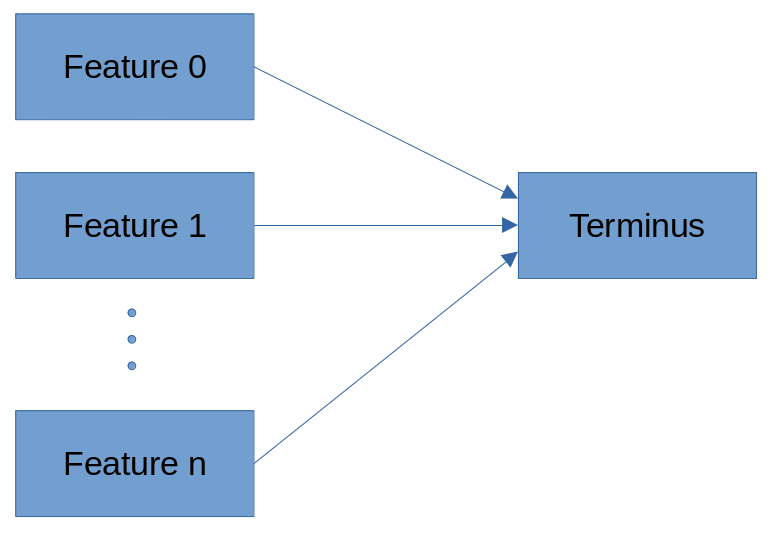
\includegraphics[width=0.7\textwidth]{images/model_fig.png}
					\caption{The general architecture format for the models used in these
					experiments. In every feature, as well as in the terminus, there can be
					various kinds of hidden layers.}
					\label{fig:model_plot}
				\end{center}
			\end{figure}
			\begin{figure}[htbp]
				\begin{center}
					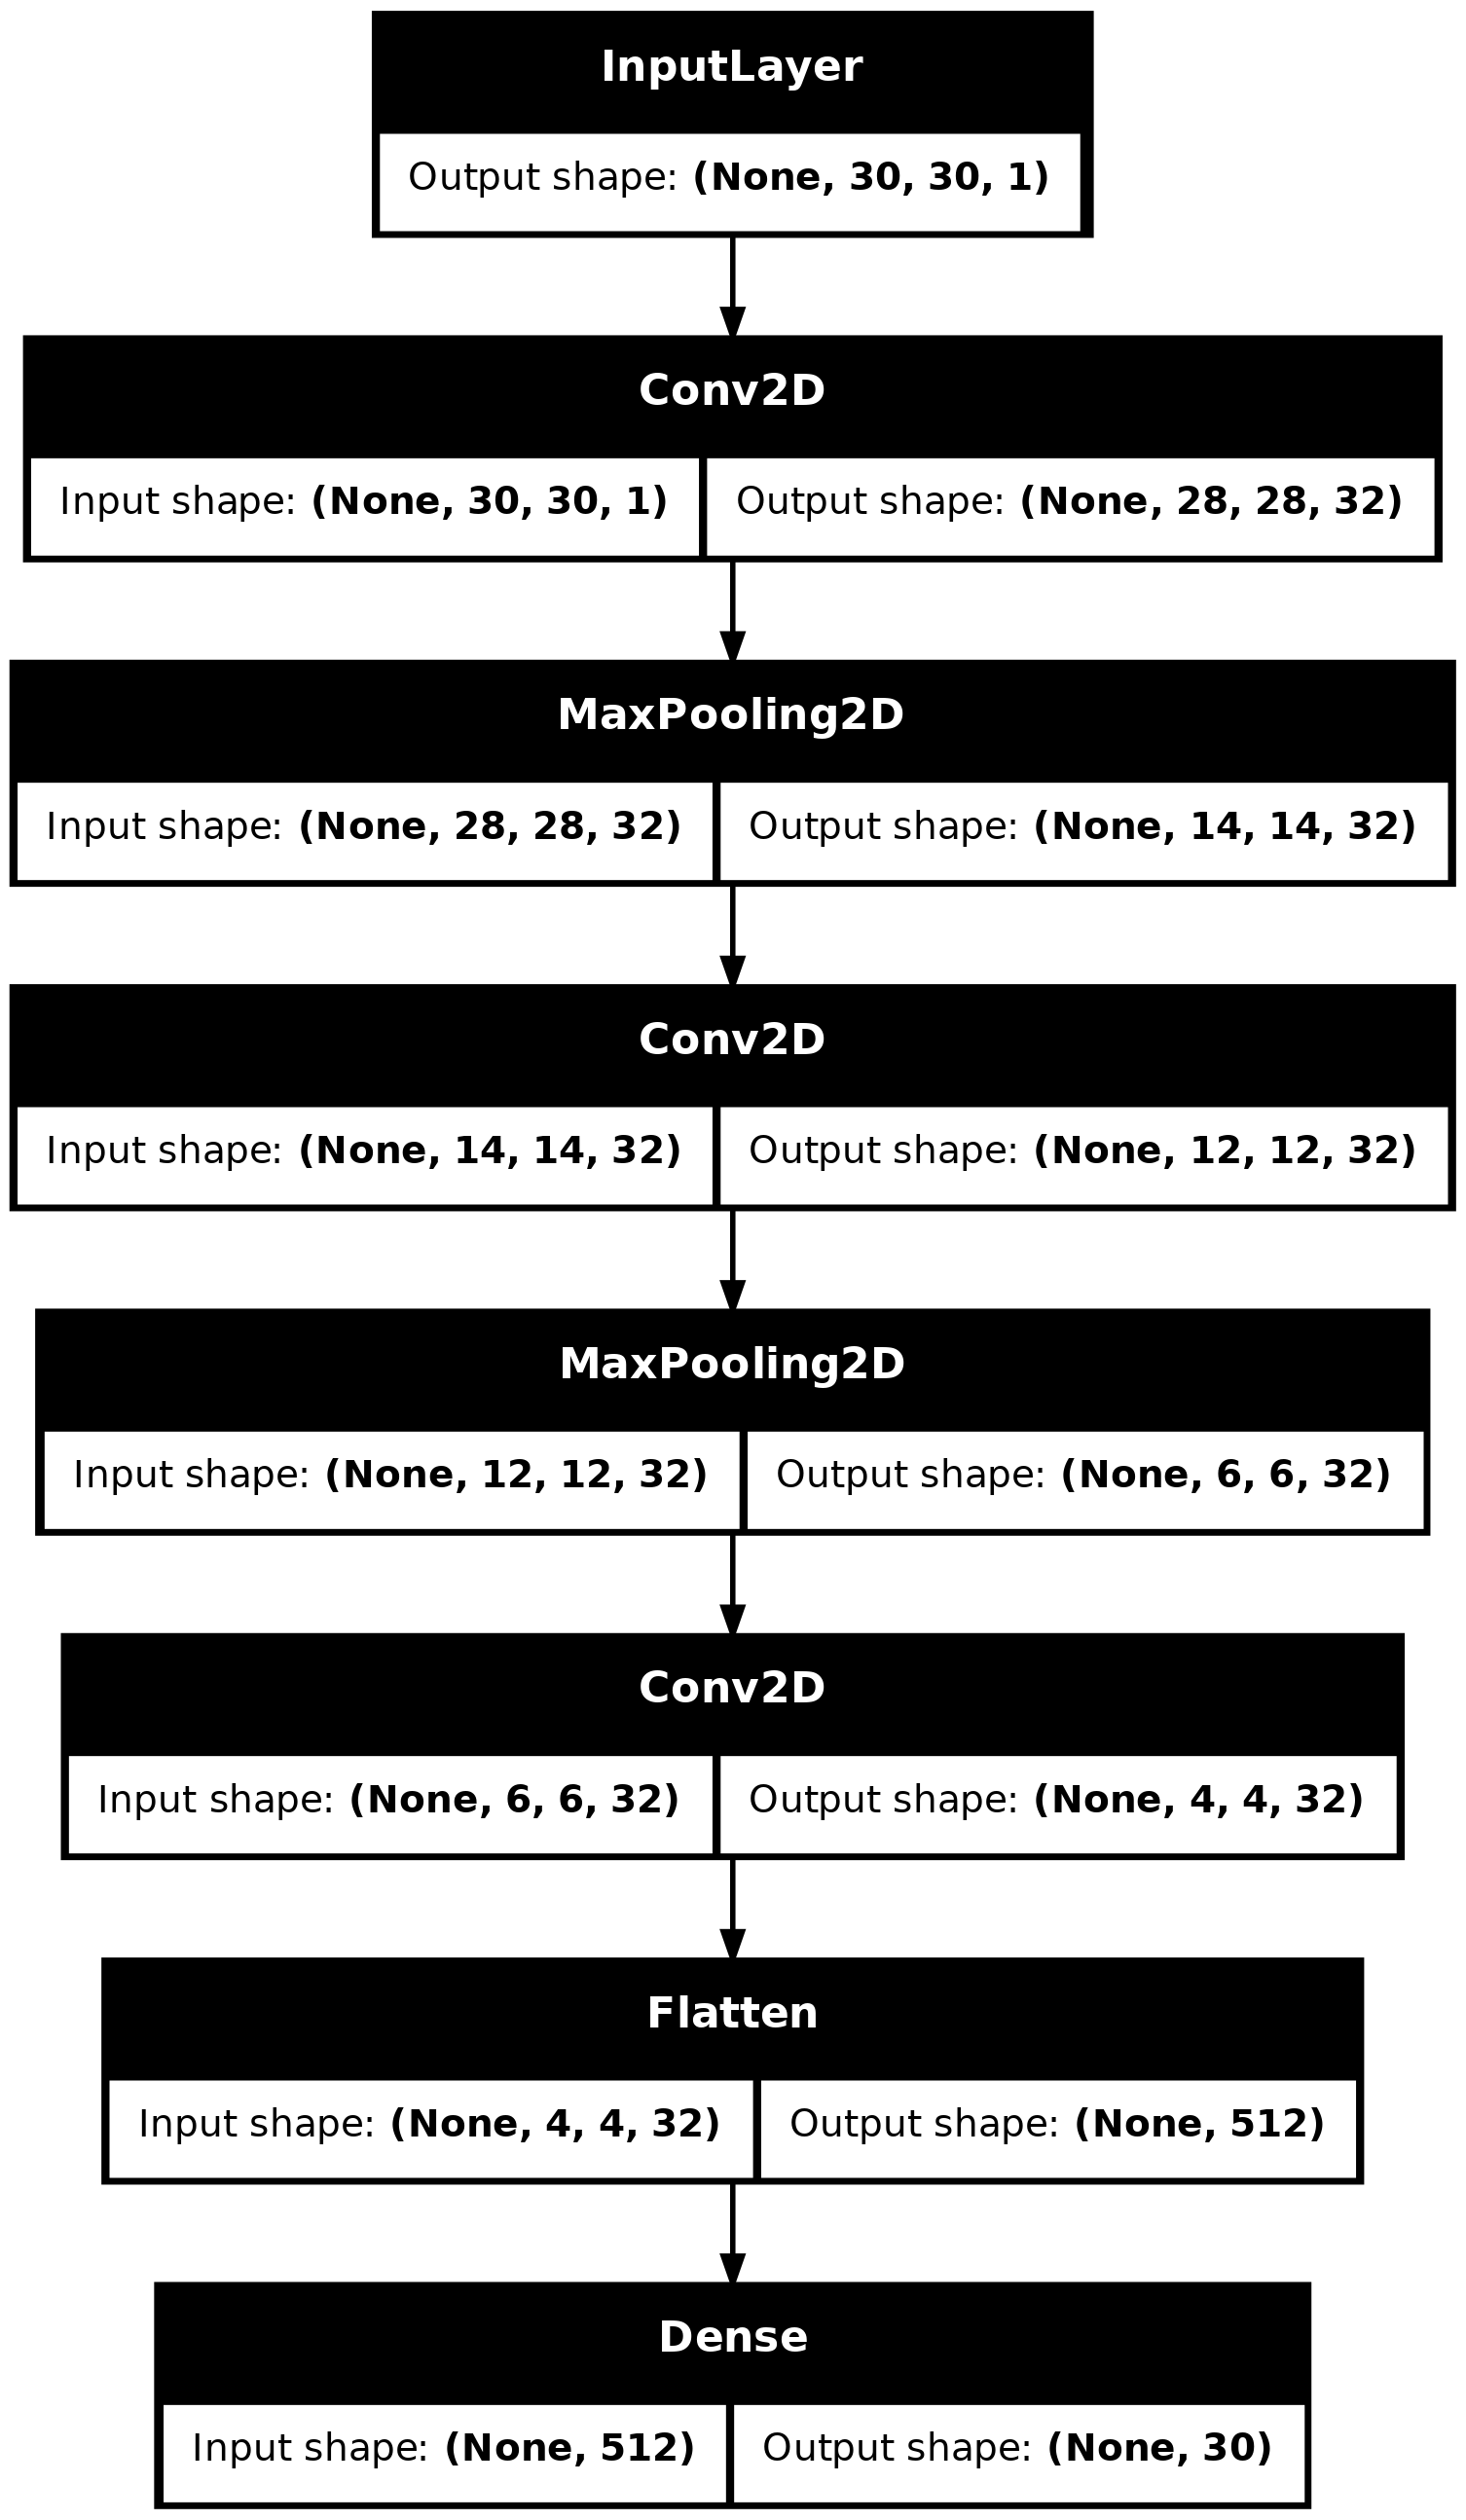
\includegraphics[width=0.4\textwidth]{images/mel_model_plot.png}
					\caption{Example of a submodel for the mel-spectrogram features, including the
					hidden layers and output sizes.}
					\label{fig:mel_model_plot}
				\end{center}
			\end{figure}
			\begin{figure}[htbp]
				\begin{center}
					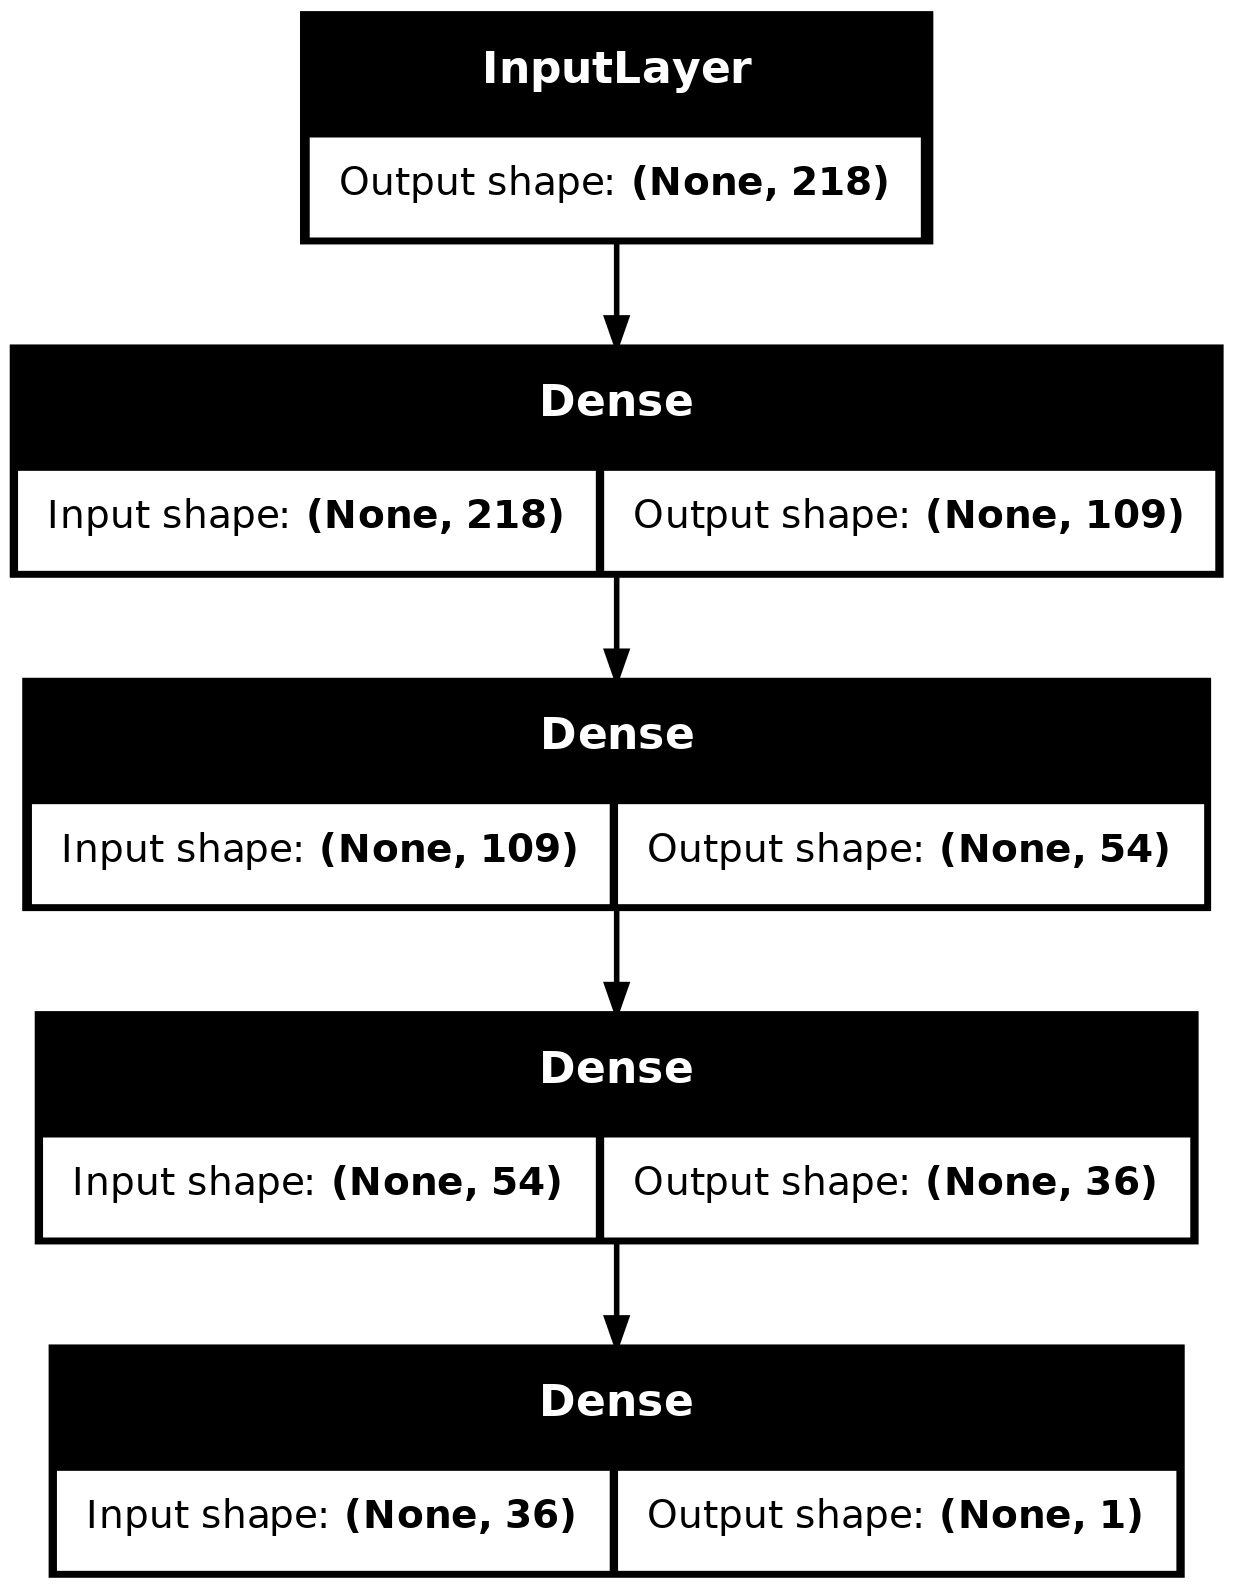
\includegraphics[width=0.4\textwidth]{images/term_model_plot.png}
					\caption{Example of a terminus model with three hidden layers.}
					\label{fig:term_model_plot}
				\end{center}
			\end{figure}
			\subsubsection{Training and Evaluation}
			The black-box model described in the previous section was trained on the first portion
			of the dataset, differing depending on the exact experiment (more details are provided
			in the next section). Evaluation was then performed on the remaining samples in the
			dataset. Training batches consisted of 100 samples each with every window position for
			each sample and an upper limit of 1,000,000 lines per batch. For each batch, either
			one or two epochs were performed. Because a single sample can have multiple input
			lines, evaluation cannot be performed on a per-line basis, but must instead be
			summarized. Two methods are possible: median and mean, with the difference in results
			being negligible in our experiments. The default threshold is 0.5, meaning that a
			result under 0.5 is a negative result and over 0.5 is a positive result. This
			threshold can however be adjusted, useful for computing certain metrics.
		\subsection{Explanations}
		The explanations using the previously described surrogate model are generated with the
		Local Interpretable Model-agnostic Explanation (LIME) method \cite{ribeiro_why_2016}. This
		section will describe in detail how individual explanations are generated at a local level
		for individual samples, as well as how the usefulness of the explanations can be evaluated
		in general.
			\subsubsection{Generation of the Explanations}
			Because of the multi-shaped nature and independence of the input layers of the model,
			the explanations cannot be generated directly from the input itself. However, because
			the sub-models are separate from one another, having no influence on each other before
			being concatenated at the terminus, only the terminus part of the model is relevant
			for assessing the importance of the features in a single evaluation. This does,
			however, present two challenges:
			\begin{itemize}
				\item There are multiple input rows per sample.
				\item The features cannot be used directly for assessment at the terminus input
					layer.
			\end{itemize}
			The first problem can be solved by taking the mean of the explanation weights of each
			feature produced by each row of the sample features. This results in an average
			contribution of each feature to the classification of the model. Because the
			end-classification of the surrogate is also a mean, the means of the LIME-results are
			an accurate representation of the aggregate influence.
			\par
			We approached the second problem by generating intermediate data for the
			LIME-evaluation. Intermediate data was generated by first decomposing the surrogate
			model into its component models, the sub-models and the terminus, and for each
			sub-model, running a prediction on the given input features. The results of the
			predictions of the sub-models were stored and used for further analysis. This was done
			not only for the sample explanation data but also for the training data, to use as an
			input for the LIME explainer.
			\par
			The results of the LIME explainer are then summarized together on a per-feature basis
			and normalized to produce a decimal number between -1 and 1 for every feature. In this
			case, a negative value implies that the given feature pushed the result of the model
			in the negative direction (i.e. not fake), while a positive value indicates the
			opposite.
			\subsubsection{Evaluation of the Explanations}
			In order to assess if the explanations have the potential to be useful to an end
			user, we pursued the goal of summarizing many explanations generated using the
			previously described method together in a meaningful way, in order to make a
			conclusion about the general usefulness of the individual features and the influence
			and potential use of the perceptible features. However, due to a lack of existing
			standardized metrics for the global evaluation of local metrics, we propose two
			metrics, with which we will make conclusions about the usefulness of this method.
			\par
			In order to contextualize the metrics, we will make the following definitions.
			\begin{itemize}
				\item Let \(S\) be the set of samples with \(s \in S\) as an element of the set.
				\item Let \(F\) be the set of features with \(f \in F\) as an element of the set.
				\item Let \(w_{fs}\) be the weight value of feature \(f\) of sample \(s\) as
					produced by the explainer.
				\item Let \(l_{s}\) be the correct label of the sample \(s\).
			\end{itemize}
			The first metric we will define is the mean of the absolute values of the weights of
			the explanations, summarized along the sample axis, delivering one value per feature.
			We will further refer to this metric as importance, and it can be mathematically
			defined as follows for every \(f \in F\):
			\[\frac{\sum_{s \in S} |w_{fs}|}{|S|}\]
			The second metric we will define is the average aggregate correctness on a per-feature
			basis, which we will further refer to as trust. The trust per feature \(f \in F\) can
			be defined as follows:
			\[\frac{\sum_{s \in S} w_{fs}(2l_{s}-1)}{|S|}\]
	\section{Experimental Results}
	Using the methods described in the previous section, we performed experiments training and
	testing the surrogate model, as well as generating many explanations for the purpose of
	aggregate evaluation. This section will first discuss the results and performance of the
	surrogate model, followed by an evaluation of the aggregated explanations.
		\subsection{Dataset}
		The dataset used for these experiments is the "In-the-Wild" dataset, one which focuses on
		the generalization of audio deepfake detection models by collecting real-world data, in
		comparison to other examples that use more controlled laboratory conditions
		\cite{muller_does_2022}. We have chosen it for these experiments because of the
		aforementioned focus on generalization, its relative recency, compared to some others and
		the fact that it has also been used previously by some other experiments, which provides a
		useful perspective against which we can compare our method.
		\subsection{Black-Box Model Results}
		\begin{table}[htbp]
			\centering\notsotiny
			\begin{tabular}{c | c | c | c | c | c}
				Terminus & Features & Training & Accuracy & EER & AUC \\
				\hline
				Simple & standard & 3474 & 95.02\% & 0.03702 & 0.90297 \\
				3 hidden layers & standard & 10000 & 96.27\% & 0.03214 & 0.81763 \\
				Simple & standard & 23833 2 epochs & 90.07\% & 0.90069 & 0.78889 \\
				Simple & standard & 10000 2 epochs & 94.43\% & 0.04408 & 0.89445 \\
				Simple & standard & 10000 & 94.28\% & 0.04840 & 0.90182 \\
				3 convolutional layers & standard & 10000 & 62.80\% & 0.37198 & 0.50051 \\
				Simple & expand pitch\-flucs & 10000 & 93.31\% & 0.05661 & 0.92727 \\
				3 hidden layers & expand pitch\-flucs & 10000 & 93.87\% & 0.05317 & 0.83263
			\end{tabular}
			\caption{Summary of the evaluation results of the experiments}
			\label{table:eval-results}
		\end{table}
		\begin{figure}[htbp]
			\centering
			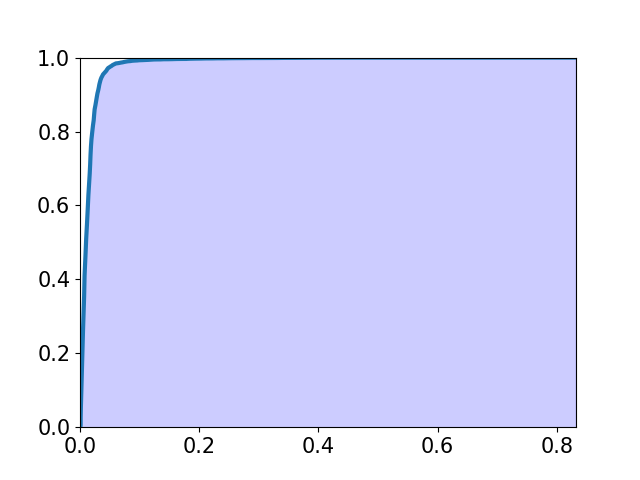
\includegraphics[width=0.7\textwidth]{images/roc_cterm.png}
			\caption{ROC curve of the best-performing model, with 3 hidden layers in the terminus
			and that standard feature set.}
			\label{fig:roc_cterm}
		\end{figure}
		\begin{figure}[htbp]
			\centering
			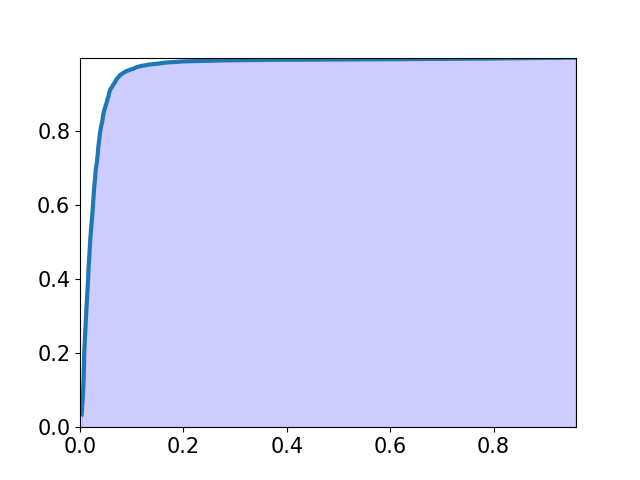
\includegraphics[width=0.7\textwidth]{images/roc_mpf.png}
			\caption{ROC curve of the model with expanded pitch fluctuation features.}
			\label{fig:roc_mpf}
		\end{figure}
		\begin{figure}[htbp]
			\centering
			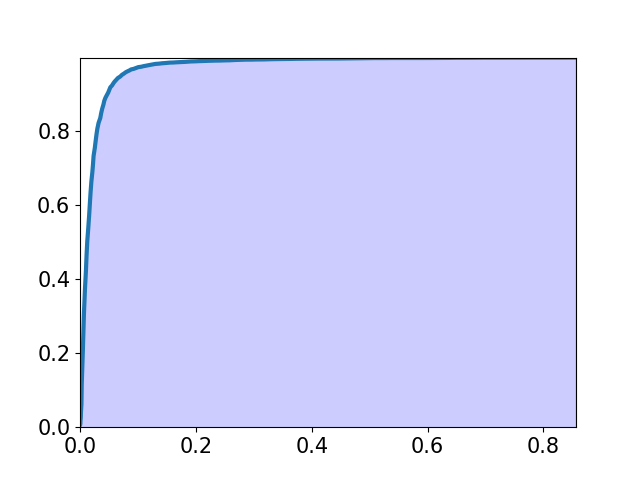
\includegraphics[width=0.7\textwidth]{images/roc_mpf_cterm.png}
			\caption{ROC curve of the model with expanded pitch fluctuation features and a
			terminus with three hidden layers.}
			\label{fig:roc_mpf_cterm}
		\end{figure}
		\sloppy
		A summary of some experiments based on the method described above is provided in table
		\ref{table:eval-results}. The table covers the type of terminus model used, where a
		"simple" terminus model does not include hidden layers, the set of features used, where
		"standard" is the feature set as described above, with expanded pitch fluctuations being
		the same feature set with the addition of pitch fluctuation features with different
		comparison distances, the training batch size and the number of epochs per batch if there
		were more than one, followed by several metrics for comparison. Figures
		\ref{fig:roc_cterm}, \ref{fig:roc_mpf} and \ref{fig:roc_mpf_cterm} depict the ROC curve of
		three of the models, which were selected for use in explanation generation in the
		following section.
		\par
		The model that achieved the best results was trained on the first
		10000 samples of the dataset and evaluated on the rest evaluated using the methods
		previously described. It has an evaluation accuracy of 96.3\% with the default threshold
		of 0.5, with an EER of approximately 0.03214. This outperforms other results tested in the
		original paper on this dataset \cite{muller_does_2022}. This result also exceeds some
		other results tested on this dataset, such as an example \cite{yang_robust_2024} produced
		using a variety of imperceptible features and trained on the ASV2019 dataset, while
		underperforming one other method \cite{ranjan_statnet_2022} that made use of raw
		waveform-based features, training on 70 percent of the data in the dataset, validating on
		10 percent and testing on the remaining 20 percent.
		\subsection{Explanation Results}
		\begin{table}[htbp]
			\centering
			\begin{tabular}{c | c | c}
				Feature & importance & trust \\
				\hline
				HNRs & 0.1140 & -0.0543 \\
				mel spectrogram & 0.1084 & -0.0378 \\
				MFCC & 0.7029 & 0.3753 \\
				f0 lengths & 0.0 & 0.0 \\
				onset strengths & 0.0 & 0.0 \\
				intensities & 0.0 & 0.0 \\
				pitch fluctuations & 0.0 & 0.0 \\
				jitter features & 0.1277 & 0.0250 \\
				shimmer features & 0.1227 & 0.0017
			\end{tabular}
			\caption{Summary of the aggregated explanation results of the best performing model}
			\label{table:exp-results-cterm}
		\end{table}
		\begin{table}[htbp]
			\centering
			\begin{tabular}{c | c | c}
				Feature & importance & trust \\
				\hline
				HNRs & 0.1072 & -0.0148 \\
				mel spectrogram & 0.0428 & -0.0187 \\
				MFCC & 0.4383 & 0.2345 \\
				f0 lengths & 0.0340 & -0.0057 \\
				onset strengths & 0.0101 & -0.0027 \\
				intensities & 0.0021 & 0.0021 \\
				pitch fluctuations & 0.0059 & 0.0020 \\
				jitter features & 0.2439 & 0.0019 \\
				shimmer features & 0.1664 & 0.0070
			\end{tabular}
			\caption{Summary of the aggregated explanation results of the model with expanded
			pitch fluctuation features}
			\label{table:exp-results-more-pitch-flucs}
		\end{table}
		\begin{table}[htbp]
			\centering
			\begin{tabular}{c | c | c}
				Feature & importance & trust \\
				\hline
				HNRs & 0.2667 & -0.0788 \\
				mel spectrogram & 0.0982 & -0.0434 \\
				MFCC & 0.2879 & 0.2408 \\
				f0 lengths & 0.1690 & -0.0521 \\
				onset strengths & 0.1384 & -0.0613 \\
				intensities & 0.1576 & -0.0504 \\
				pitch fluctuations & 0.0 & 0.0 \\
				jitter features & 0.1444 & 0.0118 \\
				shimmer features & 0.1747 & 0.0116
			\end{tabular}
			\caption{Summary of the aggregated explanation results of the model with expanded
			pitch fluctuation features and a terminus with three hidden layers}
			\label{table:exp-results-mpf-cterm}
		\end{table}
		In order to obtain a full picture of the quality of the explanations generated by this
		method, we have used selected two models from the last section and generated explanations
		on the first 500 samples of the testing data. We then summarized the explanations generated
		using both of the previously introduced metrics. A summary of the results of both metrics
		summarized by the feature is presented in tables \ref{table:exp-results-cterm},
		\ref{table:exp-results-more-pitch-flucs} and \ref{table:exp-results-mpf-cterm}. 
		\subsubsection{Best-Performing Model}
		Measuring by both metrics, the MFCCs had the most positive and the most correct influence
		on the classification results of the model, With the jitter features as a distant second
		for trust and importance. This indicates that the MFCCs had not only the most influence,
		but also the most correct influence on the result of the classification, while the other
		features had either little, no or negative influence on the classification.
		\subsubsection{Model with Expanded Pitch-Fluctuation Features}
		This model had similarly unpromising results, with the main difference being that all
		metrics have non-zero values, meaning that all the present features had an influence on
		the classifications which were used to generate the explanations. As with the previous
		model, HNRs and mel-spectrograms had negative overall trust values, with the addition of
		the onset strengths also presenting a negative value, implying that these features have
		caused more harm than good in the tested classifications.
		\subsubsection{Model with Expanded Pitch-Fluctuation Features and Complex Terminus}
		The model with multiple pitch-fluctuation features in combination with a terminus
		containing multiple hidden layers fared similarly to the other two, this time with the
		pitch fluctuations having not influence on the outcome whatsoever. Unlike the previous
		examples, the trust value of the intensities feature was negative here.
	\section{Discussion}
	In this section, we will discuss the implications of the experimental results of the previous
	sections with a special focus being placed on the results of the explanation tests as it
	relates to the potential explainability for potential end users of such a system.
		\subsection{Viability and Potential of the Explanations}
		Because of these models' inclusion of several perceptible features, we made the hypothesis
		that this method has the potential to produce explanations that can be used as the basis
		for something more presentable to an end user. As can be seen in the previous section in
		the tables \ref{table:exp-results-cterm} \ref{table:exp-results-more-pitch-flucs}, the
		perceptible features did not contribute as much to the end result of the classification as
		their imperceptible counterparts, in spite of their increased presence in the overall set
		of input features. Two features, the HNRs and the mel-spectrograms even consistently had a
		net-negative impact on the correctness of the classifications in the experiments, leaving
		the question open, if future experiments may perform better without these features. In the
		case of the best performing model, four perceptible features, f0 lengths, onset strengths,
		intensities and pitch fluctuations had an overall average influence on the classification
		of 0, measured on both metrics, indicating that the model did not learn a correlation
		between these features and the realness of audio samples in the dataset. These features
		did have an impact on the performence of the model with expanded pitch fluctuations, but
		the difference was still minimal. In spite of this, we believe that it is still worth
		investigating if other kinds of perceptible features will have more of an influence on the
		overall classification or if there are other imperceptible features that could be used in
		the place of MFCCs that may provide a better balance between classification correctness
		and a proportional influence on the end result.
		\subsection{Limitations}
		In spite of the potential that we see with this method, it does also present some
		limitations when it comes to its real-world use, aside from the shortfalls of the
		perceptible features discussed in the previous section. The first such limitation is in
		the computational performance of the model. Because of its relative size, the model
		requires relatively capable hardware in addition to several gigabytes of memory in order
		to classify samples. This means that the devices this or a similar model can run on are
		limited, and the possibility of running this or a similar model locally on a handheld
		device such as a smartphone is limited to none at the time of writing. Another limitation
		with this method is that, even though it is known that perceptible features such as the
		ones used in our method are able to be heard by the human ear and are even used in
		medicine, for example, for diagnoses \cite{chaiwongyen_deepfake-speech_2023}, it is not
		yet clear to what extent exactly these features can be understood by the average person.
		Cursory research \cite{sharevski_blind_2024} is already present into what factors humans
		use to identify fake and real audio samples, as well as their performance, but the named
		aspects of the samples have not yet been mapped to such perceptible features as the ones
		used in this method, leaving the question of the usability of such explanations open.
		Finally, we have not addressed in our experiments how the features can be presented to the
		end user. Certain implementations of LIME already have means to present their results
		graphically, but the effectiveness of such methods has yet to be studied.
	\section{Conclusion}
	To conclude, we have presented a model architecture using a combination of various features,
	perceptible and imperceptible, with the hypothesis that such a model could be used to generate
	explanations of its own results using the LIME method that are more useful to a potential end
	user who is not already familiar with the field. This model architecture resulted in a high
	level of performance in comparison to several other methods, indicating the potential for
	consistent and correct classifications. The explanations, however, were not able to produce
	the desired result, placing most of the weight on MFCCs, with most perceptible features either
	having little, no or negative impact on the end classification with the exception of jitter
	and shimmer.
	\par
	We believe that this is a method that offers a large potential, but is not useful for the
	generation of understandable explanations in its current state. We suggest, however, that this
	method could be changed and improved in the future with other features or other changes to
	base parameters that could potentially produce more useful explanations while either holding
	the accuracy high like it is now or even improving it further.
	\newpage
	\sloppy
	\printbibliography
\end{document}
